\documentclass[dvipdfmx,twoside]{jsarticle}
\usepackage{amsmath,amssymb}
\usepackage{CJKutf8}
\usepackage{okumacro}
\usepackage{booktabs}
\usepackage{array}
\usepackage{xcolor}
\usepackage{colortbl}
\usepackage{tipa}
\usepackage{tikz}
\usepackage{fancybox}
\usepackage{wasysym}
\usepackage{pifont}
\usepackage{graphicx}
\usepackage{wrapfig}
\usepackage{geometry}
\geometry{margin=2cm}
\usepackage{fancyhdr}
\usepackage{pgfplots}
\pgfplotsset{compat=1.18}
\usepackage[utf8]{inputenc}
\usepackage{CJK}
\usetikzlibrary{positioning, intersections, calc, arrows.meta, math, through, shadows}
\usepackage{tcolorbox}
\tcbuselibrary{theorems,breakable}
\usepackage{enumerate}
\usepackage{titlesec}

% 自定义subsubsection格式
\titleformat{\subsubsection}
  {\normalfont\normalsize\bfseries}
  {1.\arabic{subsubsection}}
  {1em}
  {}
% 设置页面样式
% \pagestyle{fancy}
% \fancyhf{}
% \renewcommand{\headrulewidth}{0pt}
% \fancyhead[RO]{数学–\thepage}
% \fancyhead[LE]{数学–\thepage}

% 重新定义 plain 样式
% \fancypagestyle{plain}{%
%   \fancyhf{}%
%   \renewcommand{\headrulewidth}{0pt}%
%   \fancyhead[RO]{数学-\thepage}%
%   \fancyhead[LE]{数学-\thepage}%
% }
\newtcbtheorem[]{reidai}{例題}
{fonttitle=\gtfamily\sffamily\bfseries\upshape\large,
colframe=black,colback=black!15!white,
rightrule=1pt,leftrule=1pt,bottomrule=2pt,
colbacktitle=black,theorem style=standard,breakable,arc=10pt}
{tha}
\newcommand{\kai}%解答
{\noindent
\begin{tikzpicture}[scale=0.2, baseline=2.8pt]
\draw (3.3,1) node{\large\textgt{解 答}};
\draw[thick, rounded corners=3pt,] (0,0)--(6.5,0)--(6.5,2.2)--(0,2.2)--cycle;
\end{tikzpicture}\;}
\newcommand{\shomei}%証明
{\noindent
\begin{tikzpicture}[scale=0.2, baseline=2.8pt]
\draw (3.3,1) node{\textgt{証 明}};
\draw[double,thick,rounded corners=3pt,] (0,0)--(6.5,0)--(6.5,2.2)--(0,2.2)--cycle;
\end{tikzpicture}\;}
%補足
\newcommand{\hosoku}{\noindent
\begin{tikzpicture}[scale=0.2, baseline=2.8pt]
\draw (6,1) node{\large\textgt{補足}};
\fill (0,1)--(1,0)--(2,1)--(1,2)--cycle;
\fill[gray] (1,1)--(2,0)--(3,1)--(2,2)--cycle;
\fill (2,1)--(3,0)--(4,1)--(3,2)--cycle;
\fill (10,1)--(11,0)--(12,1)--(11,2)--cycle;
\fill[gray] (9,1)--(10,0)--(11,1)--(10,2)--cycle;
\fill (8,1)--(9,0)--(10,1)--(9,2)--cycle;
\end{tikzpicture}\;}
%注意
\newcommand{\chui}{\noindent
\begin{tikzpicture}[scale=0.2, baseline=2.8pt]
\fill (0,0)--(6.5,0)--(6.5,2.2)--(0,2.2);
\draw (3.3,1) node[white]{\large\textgt{注意!}};
\draw[thick] (0,0)--(6.5,0)--(6.5,2.2)--(0,2.2)--cycle;
\end{tikzpicture}\;}
% 自定义A方框命令
\newcommand{\abb}[1]{%
\begin{tikzpicture}[baseline]
\node[draw=black, 
      rectangle, 
      minimum width=0.8cm, 
      minimum height=0.3cm, 
      fill=gray!25, 
      font=\bfseries,
      line width=1pt,
      inner sep=2pt,
      anchor=base] {#1};
\end{tikzpicture}%
}
\newcommand{\ab}[1]{%
\begin{tikzpicture}[baseline]
\node[draw=black, 
      rectangle, 
      minimum width=0.8cm, 
      minimum height=0.3cm, 
      font=\bfseries,
      line width=1pt,
      inner sep=2pt,
      anchor=base] {#1};
\end{tikzpicture}%
}

\newcommand{\maru}[1]{\tikz[baseline=-0.7ex]{
    \node[shape=circle,draw,inner sep=1pt,minimum size=5pt,anchor=center] {\footnotesize #1};}}
\definecolor{headercolor}{RGB}{220,220,220}
\definecolor{rowcolor1}{RGB}{245,245,245}
\definecolor{rowcolor2}{RGB}{255,255,255}

% \title{\vspace{-1.5cm} 2025年8月羚課文科数学月考 }
% \author{\textnosfal{Linc\ -\ 伊}}
\date{}
\begin{document}
\thispagestyle{empty}
\begin{CJK}{UTF8}{ipxm}  % 使用ipxm字体
  %月考表纸部分
\begin{center}

\vspace*{5cm}

% 学校logo

\includegraphics[width=5cm]{pics/1.jpg}

\vspace{2cm}

% 主标题
{\fontsize{24}{30}\selectfont\bfseries\sffamily
2025年8月\\
\vspace{1em}
羚課理科数学月考\\
\vspace{1em}
解答
}

\end{center}
%問題1の内容
\newpage
\section*{問題\textrm{I}}
\setcounter{page}{1}
\noindent
\textbf{問1}\qquad 2次関数 $f(x) = -x^2 + 4x + 6$ を考える。\\
\\
\\

\vspace{2em}

(1) \quad 放物線 $y = f(x)$ の頂点の座標は $\left(\ab{\textsf{A}}, \ab{\textsf{BC}}\right)$ である。

\vspace{2em}

(2) \quad 放物線 $y = f(x)$ を $x$ 軸方向に $k$,$y$ 軸方向に $-5$ だけ平行移動して得られる放物線を $y = g(x)$ とすると

\begin{align*}
g(x) = -\left(x - \ab{\textsf{D}} - k\right)^2 + \ab{\textsf{E}}
\end{align*}
\\

である。

\vspace{1em}

(3) \quad 次の文中の $\ab{\textsf{F}}$ には,この問いの下の選択肢 \maru{0}〜\maru{4} の中から,また,$\ab{\textsf{G}}$ には,この問いの下の選択肢\\
\maru{5}〜\maru{9} の中から適するものを選びなさい。また,その他の $\ab{\phantom{AA}}$ には,適する数を入れなさい。

\vspace{2em}
関数 $g(x)$ の $-1 \leq x \leq 4$ における最大値が $3$ となるような $k$ の値を求めよう。
関数 $g(x)$ の最大値は $\abb{\textsf{E}}$ であるから,$k$ は条件 $\ab{\textsf{F}}$ または $\ab{\textsf{G}}$ を満たす。

したがって

\begin{align*}
k = -\ab{\textsf{H}} - \sqrt{\ab{\textsf{I}}}, \qquad k = \ab{\textsf{J}} + \sqrt{\ab{\textsf{K}}}
\end{align*}

である。

\vspace{2em}

\begin{tabular}{ll@{\qquad}ll}
\maru{0} & $k < -5$ かつ $k^2 + 6k + 7 = 0$ & \maru{5} & $k > 2$ かつ $k^2 - 6k + 4 = 0$ \\[0.5em]
\maru{1} & $k < -5$ かつ $k^2 - 4k + 2 = 0$ & \maru{6} & $k > 2$ かつ $k^2 + 6k + 7 = 0$ \\[0.5em]
\maru{2} & $k < -3$ かつ $k^2 + 7k + 6 = 0$ & \maru{7} & $k > 2$ かつ $k^2 - 4k + 2 = 0$ \\[0.5em]
\maru{3} & $k < -3$ かつ $k^2 + 6k + 7 = 0$ & \maru{8} & $k > 4$ かつ $k^2 - 4k + 2 = 0$ \\[0.5em]
\maru{4} & $k < -3$ かつ $k^2 - 4k + 2 = 0$ & \maru{9} & $k > 4$ かつ $k^2 + 6k + 7 = 0$ \\
\end{tabular}
\newpage
\kai \\

\noindent
(1)\quad $ f(x)=-x^2+4x+6 $に対して、頂点の$x$の座標は $ -\dfrac{B}{2A} = -\dfrac{4}{-2} = 2 $ である。その$x$の座標を代入して、頂点のy座標は $ f(2) = -2^2 + 4\times 2 + 6 = 10 $ である。したがって、頂点の座標は $\left(\color{red}{2},{\color{red}{10}}\right)$ である。\\

\noindent
(2)\quad ある $y=f(x)$ とすると、そのグラフは$x$軸方向に$a$だけ平行移動し、$y$軸方向に$b$だけ平行移動したものとなる。したがって、 $ y-b=f(x-a) $となる。問題の条件によって、$x$軸方向に$k$、$y$軸方向に$-5$だけ平行移動して得られる放物線を$g(x)$とすると、$g(x) = {\color{red}{-\left(x - 2 - k\right)^2 + 10}} $ である。\\

\noindent
(3)\quad (2)の結果により、$g(x)=-\left(x - 2 - k\right)^2 + 5\leq 5$なので、$g(x)$の最大値は $5$ である。
すなわち、 $ g(x)_{max}=5\ \implies\ x=2+k $。しかし、 $ -1 \leq x \leq 4 $におけると、 $ g(x)_{max}=3 $ である。すなわち、 $ g(x)_{max}=5 $ となるような $x$ の値は $ -1\leq x\leq 4 $ に存在しないことがわかる。
したがって、 $ x $の範囲は以下の2つの場合から考えればよい。\\

\begin{figure}[htbp]
    \centering
    \begin{minipage}{0.45\textwidth}
        \centering
        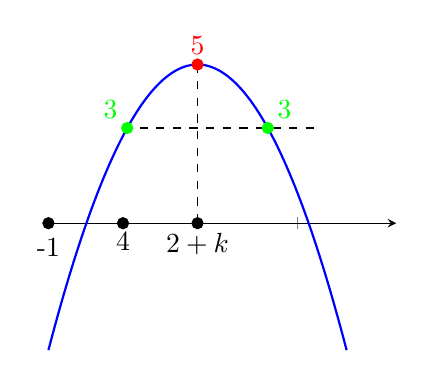
\begin{tikzpicture}
            \begin{axis}[
                axis y line=none,  % y軸を非表示
                axis x line=bottom,  % x軸のみ表示
                ymin=0, ymax=6,  % y範囲の調整
                xmin=-1, xmax=6,  % x範囲を-1から6に拡張
                width=6cm, height=4cm,
                no markers,
                xtick={-1,4},  % x=-1とx=4の目盛りを追加
                xticklabels={-1},  % ラベルをtick数に合わせ修正
                clip=false  % クリッピングを無効化(belowラベル用)
            ]
            \addplot[domain=-1:5, samples=100, thick, blue] {-(x-2)^2 + 5};  % domainをxmaxに合わせ拡張
            
            % y=5を通る垂直虚線とy=3の水平虚線
            \addplot[dashed, black] coordinates {(2,5) (2,0)};
            \addplot[dashed, black] coordinates {(0.5,3) (4.5,3)};
            
            % 点の標記
            \addplot[only marks, mark=*, mark size=2pt, red] coordinates {(2,5)};
            \addplot[only marks, mark=*, mark size=2pt, black] coordinates {(2,0)};
            \addplot[only marks, mark=*, mark size=2pt, black] coordinates {(0.5,0)};
            \addplot[only marks, mark=*, mark size=2pt, black] coordinates {(-1,0)};
            \node[above, red] at (axis cs:2,5) {5};
            \node[below, black] at (axis cs:2,0) {$2+k$};
            \node[below, black] at (axis cs:0.5,0) {$4$};
            
            % y=3の点
            \addplot[only marks, mark=*, mark size=2pt, green] coordinates {(0.5858,3) (3.4142,3)};
            \node[above left, green] at (axis cs:0.5858,3) {3};
            \node[above right, green] at (axis cs:3.4142,3) {3};
            \end{axis}
        \end{tikzpicture}
        \caption{場合1}
    \end{minipage}
    \hfill
    \begin{minipage}{0.45\textwidth}
        \centering
        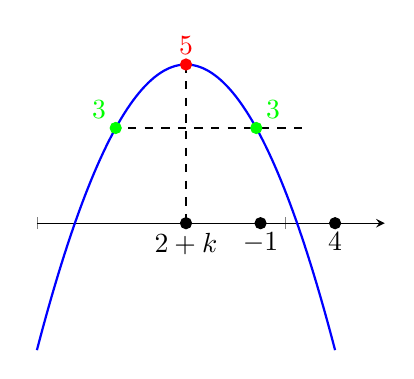
\begin{tikzpicture}
            \begin{axis}[
                axis y line=none,  % y軸を非表示
                axis x line=bottom,  % x軸のみ表示
                ymin=0, ymax=6,  % y範囲の調整
                xmin=-1, xmax=6,  % x範囲を-1から6に拡張
                width=6cm, height=4cm,
                no markers,
                xtick={-1,4},  % x=-1とx=4の目盛りを追加
                xticklabels={\empty},  % ラベルをtick数に合わせ修正
                clip=false  % クリッピングを無効化(belowラベル用)
            ]
            \addplot[domain=-1:5, samples=100, thick, blue] {-(x-2)^2 + 5};  % domainをxmaxに合わせ拡張
            
            % y=5を通る垂直虚線とy=3の水平虚線
            \addplot[dashed, black] coordinates {(2,5) (2,0)};
            \addplot[dashed, black] coordinates {(0.5,3) (4.5,3)};
            
            % 点の標記
            \addplot[only marks, mark=*, mark size=2pt, red] coordinates {(2,5)};
            \addplot[only marks, mark=*, mark size=2pt, black] coordinates {(2,0)};
            \addplot[only marks, mark=*, mark size=2pt, black] coordinates {(3.5,0)};
            \addplot[only marks, mark=*, mark size=2pt, black] coordinates {(5,0)};
            \node[above, red] at (axis cs:2,5) {5};
            \node[below, black] at (axis cs:2,0) {$2+k$};
            \node[below, black] at (axis cs:3.5,0) {$-1$};
            \node[below, black] at (axis cs:5,0) {$4$};

            % y=3の点
            \addplot[only marks, mark=*, mark size=2pt, green] coordinates {(0.5858,3) (3.4142,3)};
            \node[above left, green] at (axis cs:0.5858,3) {3};
            \node[above right, green] at (axis cs:3.4142,3) {3};
            \end{axis}
        \end{tikzpicture}
        \caption{場合2}
    \end{minipage}
\end{figure}
\ \\

\noindent
場合1では、 $ x=2+k> 4\ \implies\ k>2$ である。 $ g(x)_{max}=g(4)=3 $より、$g(4)=-(2-k)^2+5=3\ \implies\ k^2-4k+2=0 $。したがって、 {\color{red}{\maru{7}}} が正しい。\\
\indent
$k>2$におけて、$k^2-4k+2=0$を計算すると、$k=\dfrac{4\pm\sqrt{4^2-4\times 1\times 2}}{2\times 1}=\dfrac{4\pm\sqrt{8}}{2}=\dfrac{4\pm 2\sqrt{2}}{2}=2\pm \sqrt{2}$である。$k>2$によって $ k = \color{red}{2+\sqrt{2}} $ である。\\

\noindent
場合2では、 $ x=2+k< -1\ \implies\ k<-3$ である。 $ g(x)_{max}=g(-1)=3 $より、$g(-1)=-(3+k)^2+5=3\ \implies\ k^2+6k+7=0 $。したがって、 {\color{red}{\maru{3}}} が正しい。\\
\indent
$k<-3$におけて、$k^2+6k+7=0$を計算すると、$k=\dfrac{-6\pm\sqrt{6^2-4\times 1\times 7}}{2\times 1}=\dfrac{-6\pm\sqrt{36-28}}{2}=\dfrac{-6\pm\sqrt{8}}{2}=\dfrac{-6\pm 2\sqrt{2}}{2}=-3\pm \sqrt{2}$である。$k<-3$によって $ k = \color{red}{-3-\sqrt{2}} $ である。\\ 
\newpage
\noindent
\textbf{問2} \quad 大中小3個のさいころを同時に投げて出た目の数をそれぞれ $x, y, z$ とし\\
\\ 
\\

\begin{align*}
x = y = z \quad &\text{である事象を } A, \\
x + y + z = 7 \quad &\text{である事象を } B, \\
x + y = z \quad &\text{である事象を } C
\end{align*}

とする。

\vspace{3em}

(1) \quad 事象 $A, B, C$ の起こる場合の数は,それぞれ

\begin{align*}
A \text{ が } \ab{\textsf{L}}, \quad B \text{ が } \ab{\textsf{MN}}, \quad C \text{ が } \ab{\textsf{OP}}
\end{align*}

である。

\vspace{3em}

(2) \quad 事象 $A \cap B$, $B \cap C$, $C \cap A$ の起こる場合の数は,それぞれ

\begin{align*}
A \cap B \text{ が } \ab{\textsf{Q}}, \quad B \cap C \text{ が } \ab{\textsf{R}}, \quad C \cap A \text{ が } \ab{\textsf{S}}
\end{align*}

である。

\vspace{3em}

(3) \quad 事象 $B \cup C$ の起こる確率 $P(B \cup C)$ は

\begin{align*}
P(B \cup C) = \frac{\ab{\textsf{T}}}{\ab{\textsf{UV}}}
\end{align*}

である。
\newpage
\kai \\

\noindent
(1)\quad さいころの目は $1, 2, 3, 4, 5, 6$ の6通りである。したがって、$x=y=z$ の場合は $6$ 通りである。したがって、$A$の事象は ${\color{red}{6}}$ 通りである。\\

\indent
$B$の事象:\ $x+y+z=7$ に関しては、$x+y+z=7$ を満たす組み合わせを考えると、$(1, 1, 5)$は$\dfrac{3!}{2!1!}=3$通り ,$(1, 2, 4)$は$\dfrac{3!}{1!1!1!}=6$通り, $(3, 3,1)$は$\dfrac{3!}{2!1!}=3$通り, $(2, 2, 3)$は$\dfrac{3!}{2!1!}=3$通りなどがある。これらの組み合わせを全て列挙すると、$B$の事象は ${\color{red}{15}}$ 通りである。\\

\indent
$C$の事象:\ $x+y=z$ に関しては、$z$の範囲を絞っておくと、$2\leq z \leq 6$ である。よって、$z$の値ごとに場合分けをすると、\\
$z=2$ の場合:\ $x+y=2$ となる組み合わせは $(1, 1, 2)$ のみである。したがって、$1$ 通りである。\\
$z=3$ の場合:\ $x+y=3$ となる組み合わせは $(1, 2, 3)$と$(2,1,3)$ である。したがって、$2$ 通りである。\\
$z=4$ の場合:\ $x+y=4$ となる組み合わせは $(2, 2, 4), (1, 3, 4),(3,1,4)$ である。したがって、$3$ 通りである。\\
$z=5$ の場合:\ $x+y=5$ となる組み合わせは $(2, 3, 5), (3, 2, 5),(1, 4, 5),(4, 1, 5)$ である。したがって、$4$ 通りである。\\
$z=6$ の場合:\ $x+y=6$ となる組み合わせは $(3, 3, 6), (2, 4, 6),(4, 2, 6),(1, 5, 6),(5, 1, 6)$ である。したがって、$5$ 通りである。以上より、$C$の事象は ${\color{red}{15}}$ 通りである。\\

\noindent
(2)\quad $A \cap B$ の事象は ${\color{red}{0}}$ 通りである。$B\cap C$の事象は${\color{red}{0}}$ 通りである。$C\cap A$の事象は${\color{red}{0}}$ 通りである。\\

\noindent
(3)\quad 全ての事象の場合の数は$6\times 6\times 6=6^3=216$通りである。したがって、$P(B)=\dfrac{15}{216}$, $P(C)=\dfrac{15}{216}$, \\[0.5em]
$P(B \cap C) = 0$ である。$P(B \cup C) = P(B) + P(C) - P(B \cap C)$によって、$P(B \cup C) = \dfrac{15}{216} + \dfrac{15}{216} - 0 = \dfrac{30}{216} = \color{red}{\dfrac{5}{36}}$\\

\hosoku\\

\noindent
事象 A, B が生じる確率をそれぞれ P(A), P(B) とおくと、和集合の確率について

\[ P(A \cup B) = P(A) + P(B) - P(A \cap B) \]

\indent
が成り立つ。\\

\shomei\\

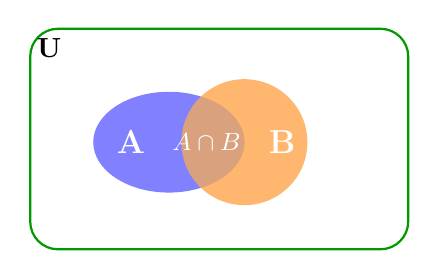
\begin{tikzpicture}[scale=0.8]
    % 全体集合Uの枠(角丸長方形)
    \draw[thick, green!60!black, rounded corners=10pt] 
        (-3, -2) rectangle (3, 1.5);
    
    % 全体集合Uのラベル
    \node at (-2.7, 1.2) {\textbf{U}};
    
    % 集合A(青い楕円)- 位置を少し右に移動して重なりを拡大
    \fill[blue!70, opacity=0.7] (-0.8, -0.3) ellipse (1.2 and 0.8);
    
    % 集合B(オレンジ色の円)- 位置を少し左に移動して重なりを拡大
    \fill[orange!80, opacity=0.7] (0.4, -0.3) circle (1);
    
    % 交集合部分の色調整(重なり部分を暗くする)
    \begin{scope}
        \clip (-0.8, -0.3) ellipse (1.2 and 0.8);
        \fill[brown!60, opacity=0.5] (0.4, -0.3) circle (1);
    \end{scope}
    
    % 集合Aのラベル(白文字)- 位置を調整
    \node[white, font=\large\bfseries] at (-1.4, -0.3) {A};
    
    % 集合Bのラベル(白文字)- 位置を調整
    \node[white, font=\large\bfseries] at (1.0, -0.3) {B};
    
    % 交集合部分のラベル(A∩B)
    \node[white, font=\small\bfseries] at (-0.2, -0.3) {$A \cap B$};
    
\end{tikzpicture}
\\

\noindent
事象 $A, B$ の関係は上の図のようになります($U$ は全事象)。\\

\noindent
確率を面積として捉えると、$A \cup B$ に相当する面積を求めるためには、$A, B $の面積を足した後、$A \cap B$ の面積を引けばよいことがわかる。
\newpage
\section*{問題\textrm{II}}
\setcounter{page}{1}
\noindent
\textbf{問1} \quad 2つのベクトル $\vec{a}$ と $\vec{b}$ のなす角は $60°$ であり,$|\vec{a}| = 1$,$|\vec{b}| = 2$ とする。また,実数 $x$ に対して,$\vec{u} = x\vec{a} + \vec{b}$,$\vec{v} = x\vec{a} - \vec{b}$ とする。$x > 1$ のとき,$\vec{u}$ と $\vec{v}$ のなす角が $45°$ となるような $x$ の値を求めよう。以下,$\vec{u} \cdot \vec{v}$ は $\vec{u}$ と $\vec{v}$ の内積を表し,$\vec{a} \cdot \vec{b}$ は $\vec{a}$ と $\vec{b}$ の内積を表す。

\vspace{2em}
まず,ベクトル $\vec{u}$ と $\vec{v}$ のなす角は $45°$であるから

\begin{align*} 
\left(\vec{u} \cdot \vec{v}\right)^2 = \frac{\ab{\textsf{A}}}{\ab{\textsf{B}}} |\vec{u}|^2 |\vec{v}|^2
\end{align*}

\noindent
を得る。$\vec{a} \cdot \vec{b} = \ab{\textsf{C}}$ であることに注意して,この式を $x$ で表すと

\begin{align*}
x^4 - \ab{\textsf{DE}} x^2 + \ab{\textsf{FG}} = 0
\end{align*}

\noindent
となる。これを変形して

\begin{align*}
\left(x^2 - \ab{\textsf{H}}\right)^2 = \left(\ab{\textsf{I}} \sqrt{\ab{\textsf{J}}} x\right)^2
\end{align*}

\noindent
を得る。

したがって,$x > 1$ に注意して,これを解くと

$$
x = \sqrt{\ab{\textsf{K}}} + \sqrt{\ab{\textsf{L}}}
$$

となる。
\newpage
\kai \\

\noindent
(1)\quad 最初は$\vec{u}$と $\vec{v}$ の内積を求めると、$\vec{u}\cdot\vec{v}=|\vec{u}|\cdot|\vec{v}|\cos(45°)=\dfrac{\sqrt{2}}{2}|\vec{u}||\vec{v}|$となる。したがって、$(\vec{u}\cdot\vec{v})^2=(\dfrac{\sqrt{2}}{2}|\vec{u}||\vec{v}|)^2=\color{red}{\dfrac{1}{2}}|\vec{u}|^2|\vec{v}|^2$となる。\\

\noindent
(2)\quad $\vec{a} \cdot \vec{b}$に関しては、$\vec{a} \cdot \vec{b} = |\vec{a}||\vec{b}|\cos(60°)=1\times 2\times \dfrac{1}{2}= {\color{red}{1}}$となる。\\

\noindent
(3)\quad $\vec{u} \cdot \vec{v}$を求めると、$\vec{u} \cdot \vec{v} = (x\vec{a} + \vec{b}) \cdot (x\vec{a} - \vec{b}) = x^2(\vec{a} \cdot \vec{a}) - (\vec{b} \cdot \vec{b}) = x^2|\vec{a}|^2 - |\vec{b}|^2 = x^2 - 4$となる。\\

\noindent
(4)\quad $\vec{u}$と$\vec{v}$の大きさを求めると、$|\vec{u}|^2 = |x\vec{a} + \vec{b}|^2 = |x\vec{a}|^2 + |\vec{b}|^2 + 2(x\vec{a} \cdot \vec{b}) = x^2 + 4 + 2x(\vec{a} \cdot \vec{b})$となる。したがって、$|\vec{u}|^2 = x^2 + 2x +4$となる。$\vec{v}$の大きさは同様に求めることができ、$|\vec{v}|^2 = x^2 - 2x + 4$となる。したがって、\\[0.5em]

$\begin{cases}
|\vec{u}|^2 = x^2 + 2x + 4 \\
|\vec{v}|^2 = x^2 - 2x + 4\\
\vec{u} \cdot \vec{v} = x^2 - 4
\end{cases}$を$(\vec{u}\cdot\vec{v})^2 = \dfrac{1}{2}|\vec{u}|^2|\vec{v}|^2$に代入すると、$\color{red}{x^4-20x^2+16=0}$を得る。\\

\noindent
(5)\quad $x^4-20x^2+16=0$を変形すると、$\left(x^2 - 4\right)^2-12x^2 =0\ \implies\ \left(x^2 - {\color{red}{4}}\right)^2 = \color{red}{\left(2\sqrt{3}x\right)^2}$となる。したがって、$x^2 - 4 = \pm 2\sqrt{3}x$となる。\\

\noindent
(6)\quad $x^2 - 4 = 2\sqrt{3}x$を解くと、$x^2 - 2\sqrt{3}x - 4 = 0$となる。したがって、$x = \dfrac{2\sqrt{3} \pm \sqrt{(2\sqrt{3})^2 + 16}}{2} = \sqrt{3} \pm \sqrt{7}$となる。$x > 1$に注意して、$x = \color{red}{\sqrt{3} + \sqrt{7}}$となる。$x^2-4 = -2\sqrt{3}x$を解くと、$x^2 + 2\sqrt{3}x - 4 = 0$となる。\\[0.5em]
したがって、$x = \dfrac{-2\sqrt{3} \pm \sqrt{(2\sqrt{3})^2 + 16}}{2} = -\sqrt{3} \pm \sqrt{7}$となる。$x > 1$に注意して、$x = -\sqrt{3} + \sqrt{7}<1$となるので、これは解ではない。\\
\newpage
\noindent
\textbf{問2} \quad 複素数平面上で,$z^3$ が実数となるような複素数 $z$ を考える。\\
\\

\vspace{2em}

(1)\quad 上の条件を満たす複素数 $z = x + iy$ が描く図形を $C$ とする。その複素数 $z$ の偏角は

\begin{align*}
\arg z = \frac{\pi}{\ab{\textsf{M}}} k \quad (k \text{ は整数})
\end{align*}

を満たすので,図形 $C$ は $x, y$ の方程式

\begin{align*}
y = \ab{\textsf{N}}, \quad y = \sqrt{\ab{\textsf{O}}} x, \quad y = -\sqrt{\ab{\textsf{P}}} x
\end{align*}

で表される3直線である。\\


\vspace{2em}

(2) \quad $C$ 上に $|z - 2 - 2i| = r$ を満たす複素数 $z$ がただ1個だけ存在するとする。このとき,$r$ の値は

\begin{align*}
r = \sqrt{\ab{\textsf{Q}}}- \ab{\textsf{R}}
\end{align*}
\\

となる。また,そのときの $z$ の値は

\begin{align*}
z = \frac{\ab{\textsf{S}} + \sqrt{\ab{\textsf{T}}}}{\ab{\textsf{U}}} \left(1 + \sqrt{\ab{\textsf{V}}} i\right)
\end{align*}

である。

\end{CJK}
\end{document}